\documentclass[a4paper]{article}

% Packages
\usepackage[margin = 1 in]{geometry}
\usepackage{fancyhdr}
\usepackage{lastpage}
\usepackage{ctex}
\usepackage[utf8]{inputenc} % Required for inputting international characters
\usepackage[english]{babel}
\usepackage[T1]{fontenc} % Output font encoding for international characters
\usepackage[sfdefault]{ClearSans} % Use the Clear Sans font (sans serif)
\usepackage{graphicx}
\usepackage{caption}
\usepackage{subcaption}
\usepackage{float}
\usepackage{amsmath}
\usepackage{amsfonts}
\usepackage{enumitem}
\usepackage{hyperref}
\usepackage{titlesec}
\usepackage{lipsum}
\usepackage{geometry}
\usepackage{tocloft} 

\pagestyle{fancy}
% Formatting
\geometry{margin=1in}
\setlength{\parindent}{0pt}
\setlength{\parskip}{1em}
\renewcommand{\baselinestretch}{1.5}
\renewcommand{\cftsecleader}{\cftdotfill{\cftdotsep}}
\rhead{\thepage}



\begin{document}
%----------------------------------------------------------------------------------------
%	TITLE PAGE
%----------------------------------------------------------------------------------------

\begin{titlepage}
	
	\rule{\linewidth}{5pt}
	\raggedleft
	\fontsize{38pt}{50pt}\selectfont
    \textbf{\\Team Project\\}
    \fontsize{28pt}{60pt}\selectfont 
    for\\
    \fontsize{38pt}{60pt}\selectfont 
    \textbf{Submission 3\\}
	
	\vfill % Space between the title box and author information
	
	%------------------------------------------------
	%	Author name and information
	%------------------------------------------------
	
	\parbox[t]{0.93\textwidth}{ % Box to inset this section slightly
		\raggedleft % Right align the text
		\large % Increase the font size
		{\Large By Team 23-22}\\[4pt] % Extra space after name
		Zijun Li\_2272583\_zxl183\\
	}
	
\end{titlepage}
\newpage
\begin{minipage}{\textwidth}
\section{Screenshots of the vertically sliced features: To-do List}
\begin{figure}[H]
  \centering
  % First row
  \begin{minipage}{0.5\textwidth}
    \centering
    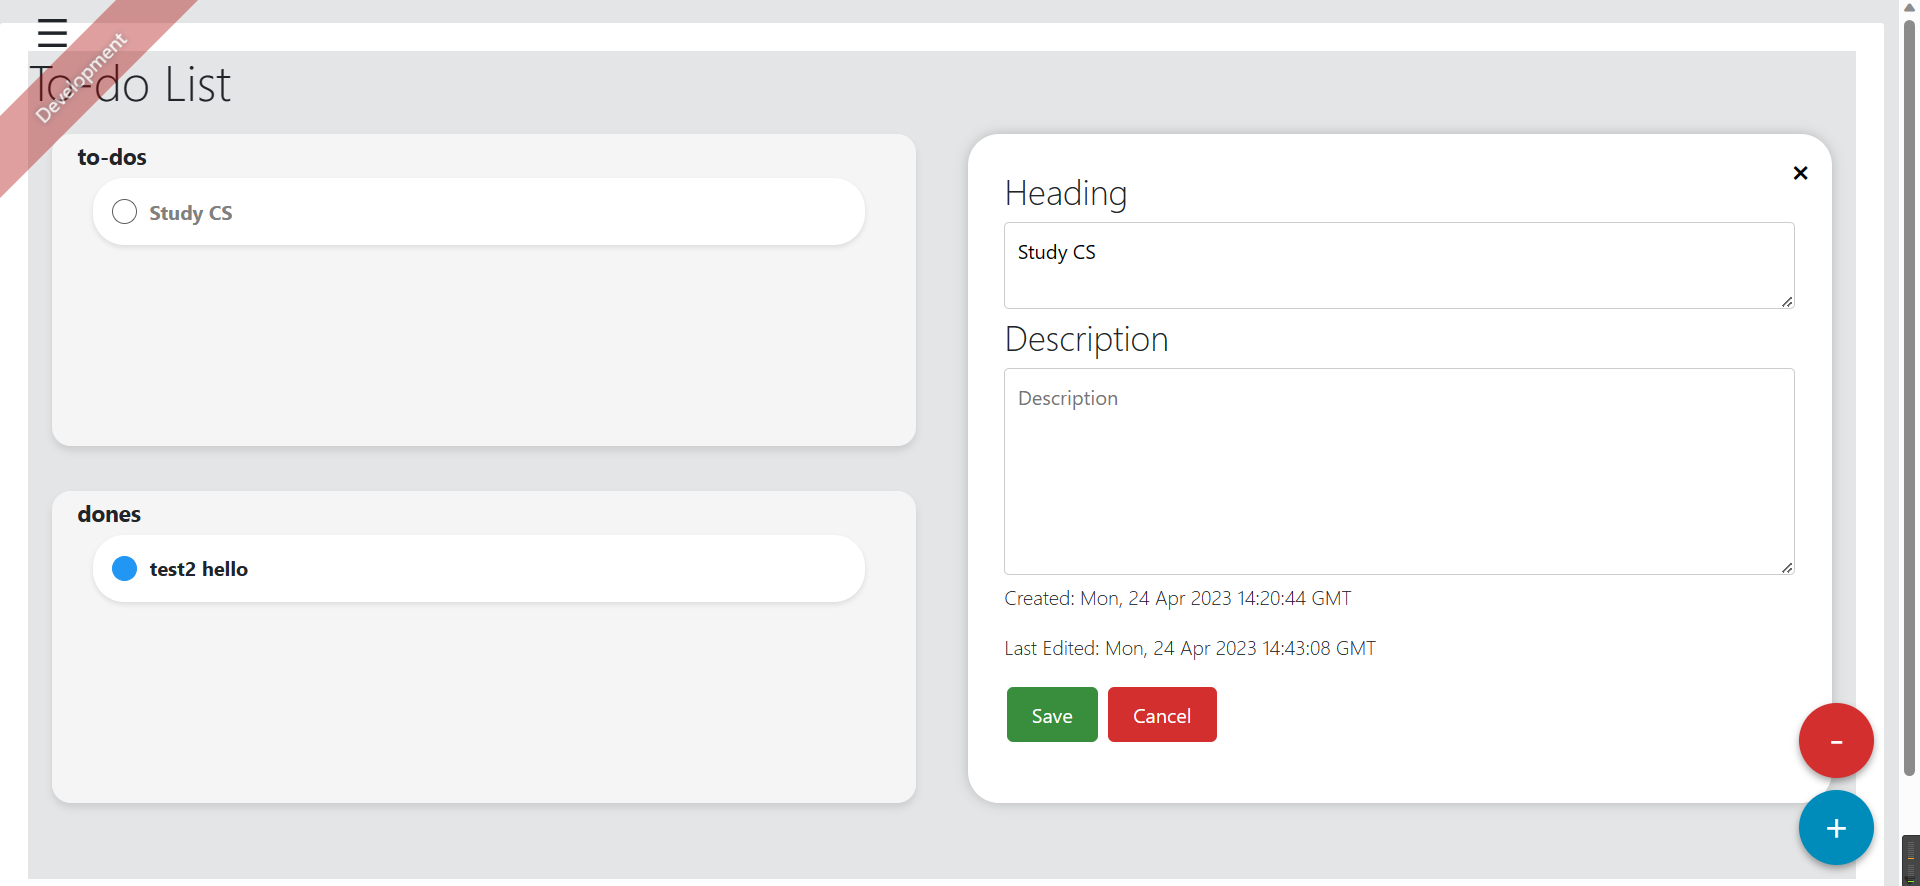
\includegraphics[width=\linewidth]{./images/Interface_Details.png} 
  \end{minipage}\hfill
  \begin{minipage}{0.5\textwidth}
    \centering
    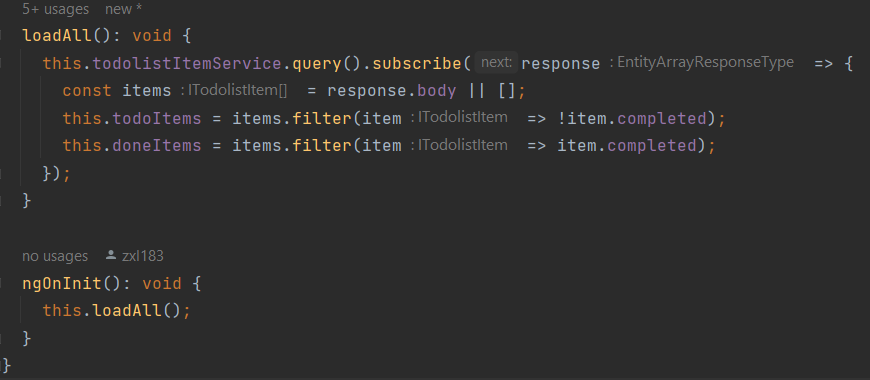
\includegraphics[width=\linewidth]{./images/Backend.png}
  \end{minipage}
  Todos/Dones: Load all items and when item is selected, its details will be shown in detail window
  
  % Second row
  \begin{minipage}{0.6\textwidth}
    \centering
    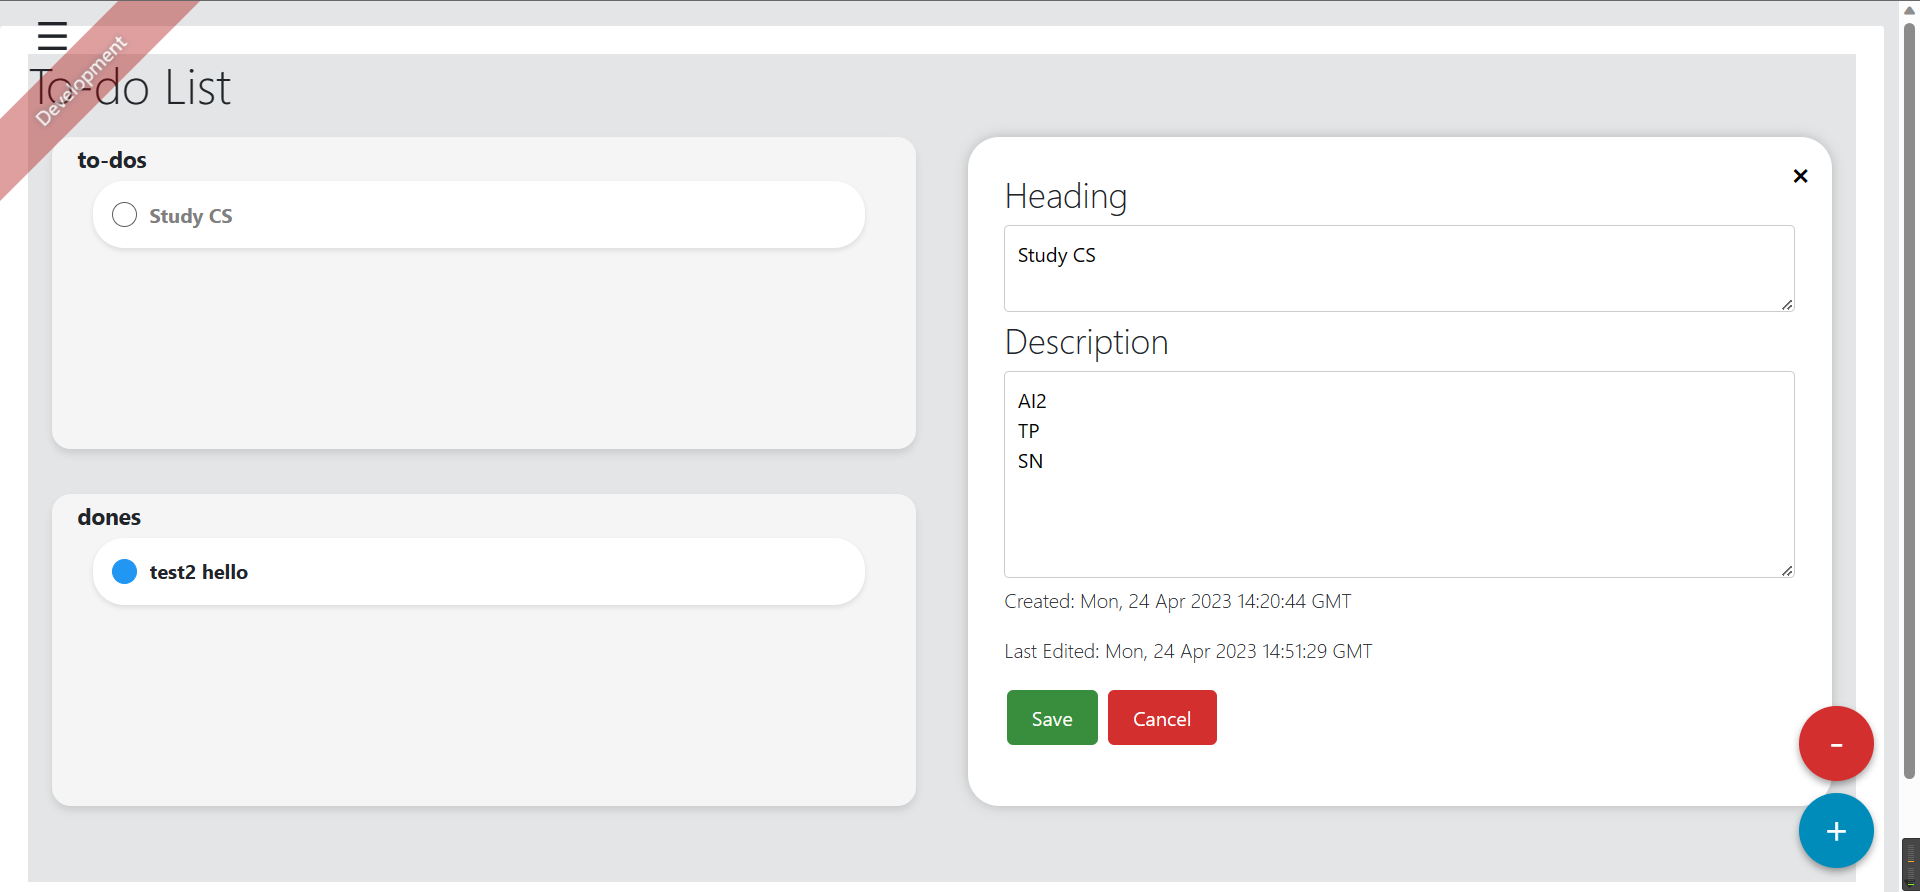
\includegraphics[width=\linewidth]{./images/Interface_Edit.png} 
  \end{minipage}\hfill
  \begin{minipage}{0.4\textwidth}
    \centering
    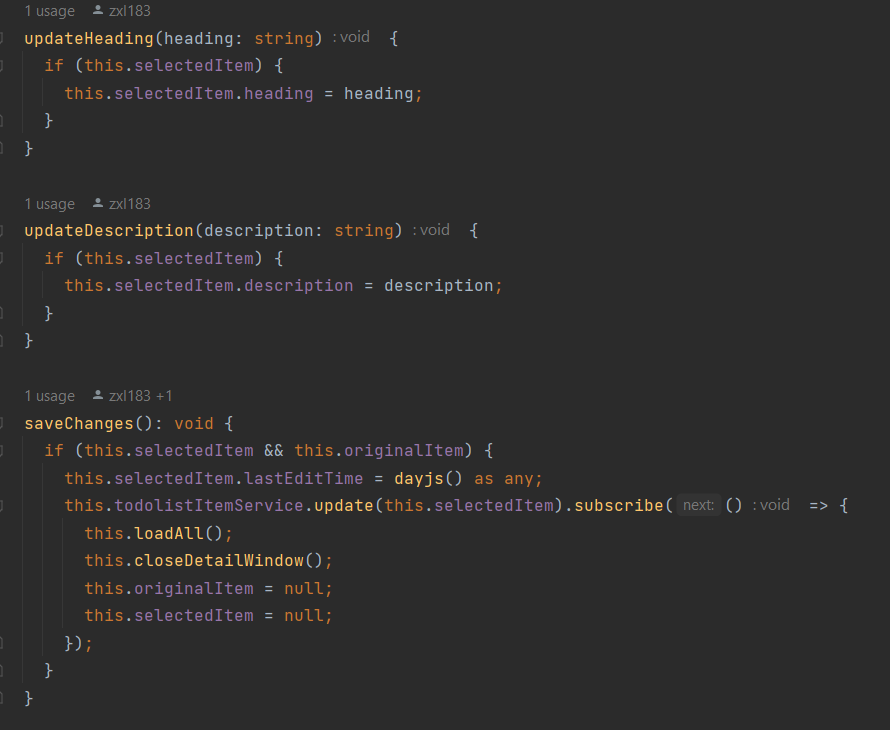
\includegraphics[width=\linewidth]{./images/Backend_Edit.png}
  \end{minipage}
  Edition: Use detail window to edit the content and save/cancel
  
  % Third row
  \begin{minipage}{0.59\textwidth}
    \centering
    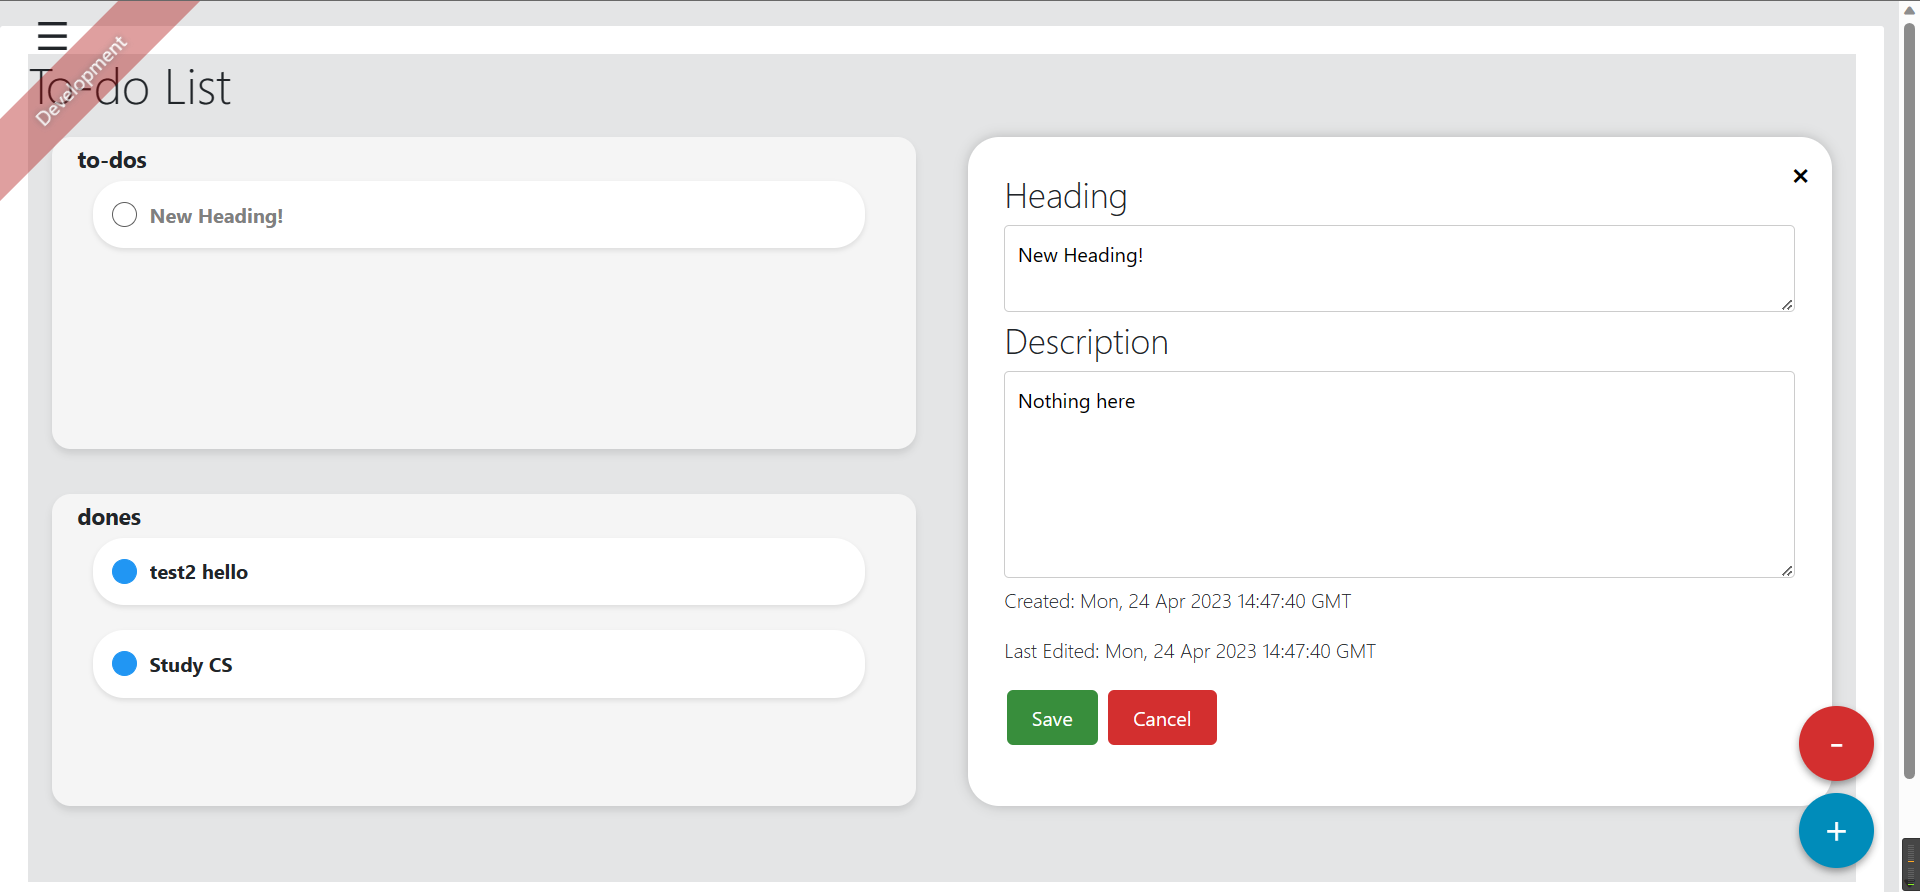
\includegraphics[width=\linewidth]{./images/Interface_Addition.png} 
  \end{minipage}\hfill
  \begin{minipage}{0.41\textwidth}
    \centering
    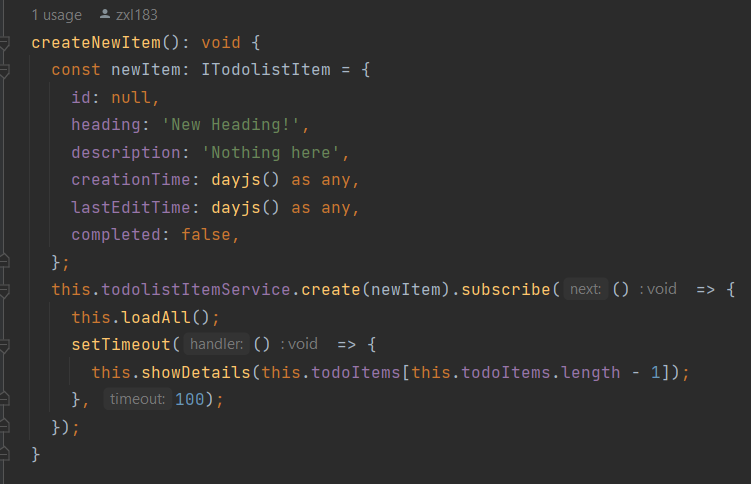
\includegraphics[width=\linewidth]{./images/Backend_Addition.png}
  \end{minipage}
  Addition: Click the Blue round button to create a new todo
  
  % Fourth row
  \begin{minipage}{0.42\textwidth}
    \centering
    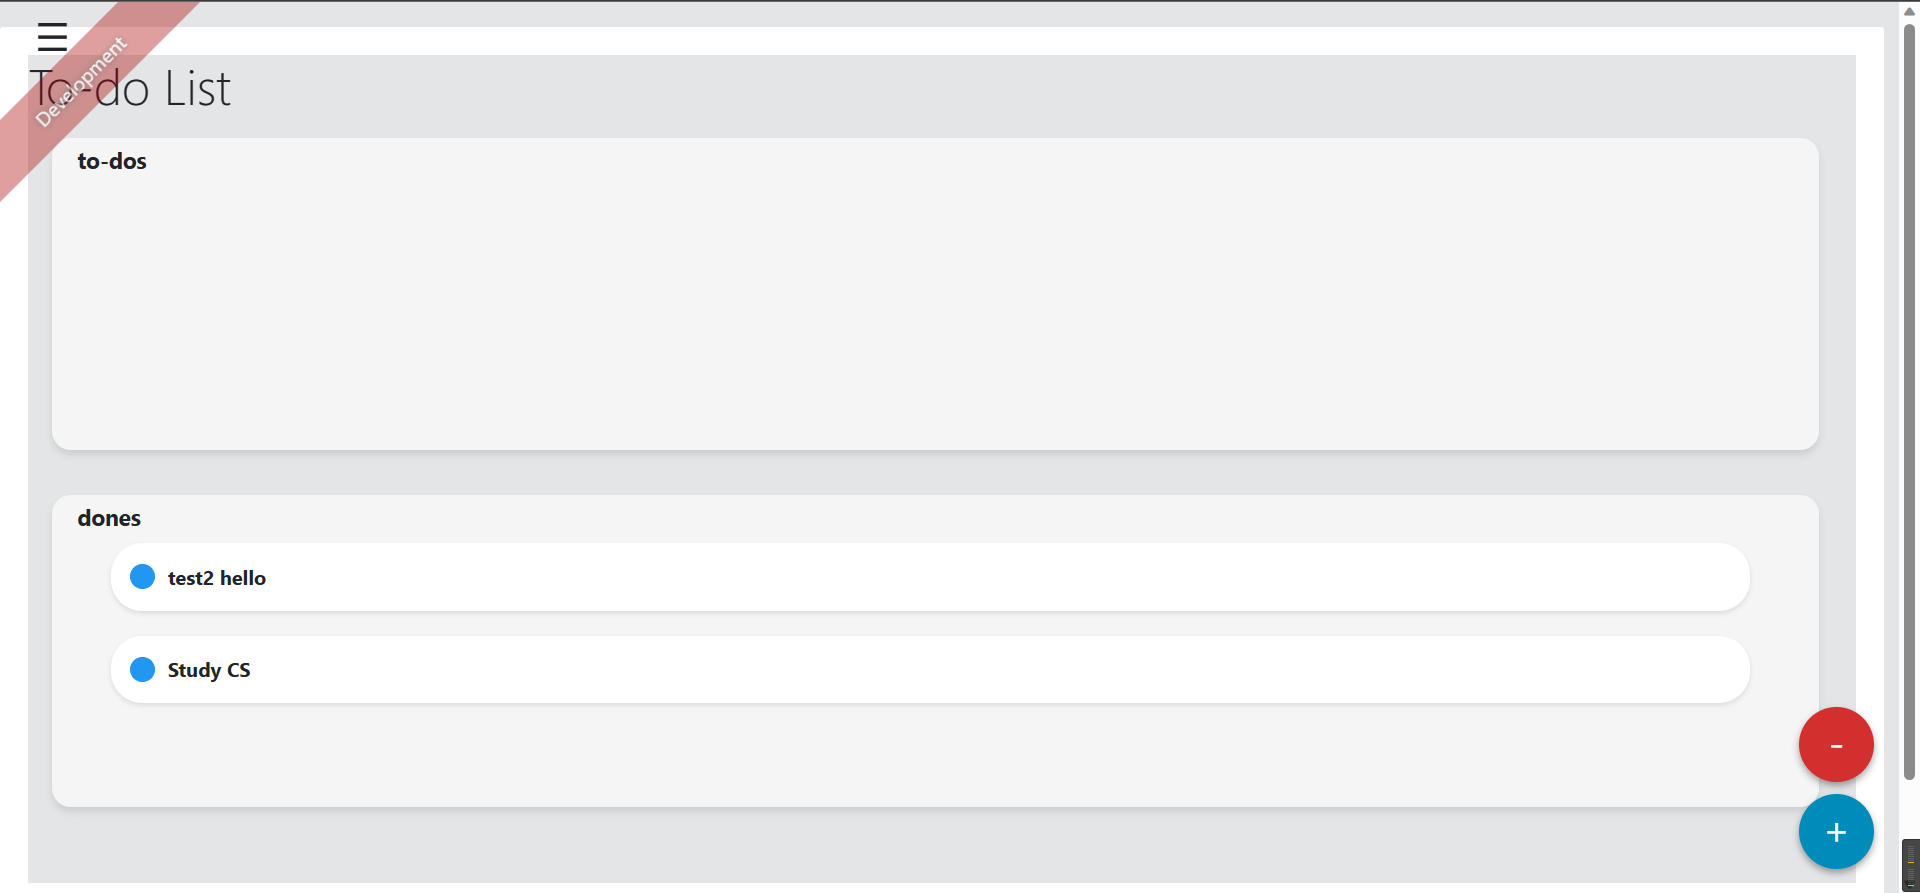
\includegraphics[width=\linewidth]{./images/Interface_Delete.png} 
  \end{minipage}\hfill
  \begin{minipage}{0.58\textwidth}
    \centering
    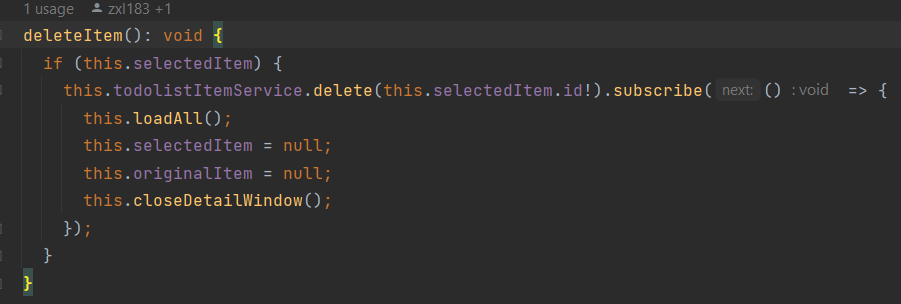
\includegraphics[width=\linewidth]{./images/Backend_Delete.png}
  \end{minipage}
  Deletion: Click the Red round button to delete the selected item

  % Fifth row
  \begin{minipage}{0.5\textwidth}
    \centering
    \includegraphics[width=\linewidth]{./images/JDL_TOdoList.png} 
  \end{minipage}\hfill
  \begin{minipage}{0.5\textwidth}
    \centering
    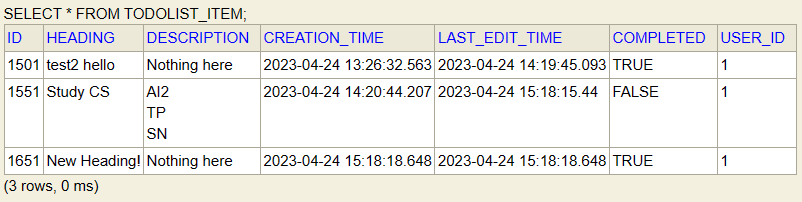
\includegraphics[width=\linewidth]{./images/Database.png}
  \end{minipage}
  Database

\end{figure}
\end{minipage}

\newpage
\section{Description of the development and integration of To-do List feature}

I developed a to-do list feature within the Time Management application. This feature can display to-do and done items from the database, toggle their completion status, add new items, delete old items, and modify their content.

We used JHipster for development, which has already integrated many features, making it very easy to create entities that connect to the database.



First, I used a JDL file to create a to-do list item entity connected to the user \href{https://git.cs.bham.ac.uk/team-projects-2022-23/team23-22/-/commit/72ab4910e6f8cb736062106f8eb215b73dd6bccb}{(Commit)}. This established a relationship between the user entity and the to-do list item entity in the backend, defining the necessary fields and database schema for the to-do list items.

Then, I modified some Java files based on this, allowing users to display only their own items instead of all items \href{https://git.cs.bham.ac.uk/team-projects-2022-23/team23-22/-/commit/c8833aae6fdc3d7390659155b1eab6a9e4fc96e5}{(Commit)}. I updated the backend service layer and repository to fetch to-do list items filtered by the user, ensuring that each user only has access to their own items.

Next, by adding and modifying TypeScript files, I implemented the switch between to-do and done items, as well as the modification, saving, and canceling of item content \href{https://git.cs.bham.ac.uk/team-projects-2022-23/team23-22/-/commit/81c0ab748310b8ee97757cc85d779b9cc70da6e6}{(Commit)}. I updated the frontend components and services to handle these actions and communicate with the backend API. This allowed the frontend to display, update, and switch the status of items, while the backend took care of persisting the changes in the database.

This comprises the content of MVP\_TodoList.

After that, I added the functionality for adding \href{https://git.cs.bham.ac.uk/team-projects-2022-23/team23-22/-/commit/fbd8b6dd71adf9d4019cfcf248393c32c3583684}{(Commit)} and deleting \href{https://git.cs.bham.ac.uk/team-projects-2022-23/team23-22/-/commit/8c186f9af83cc6132600a6bf85adcb36ae614f54}{(Commit)} items and further improved the aesthetics of the user interface. I extended the frontend components and services to include add and delete actions, while updating the backend API to handle these new requests. As a result, the frontend can now send requests to add or delete items, and the backend takes care of creating or removing records in the database accordingly.

\end{document}